
For each of the general covariance structures outlined in the previous simulation study description, data were simulated according to multivariate normal distributions with the following covariance matrices: 
\begin{enumerate} \label{simulation-model-list}
\item\label{item:cov-type-1} Mutual independence: $\Sigma = \mathrm{I}$, where 
\begin{align*}
\phi\left(t,s\right) &= 0, \quad 0 \le s < t \le 1,\\ 
\sigma^2\left(t\right) &= 1, \quad 0 \le t \le 1.
\end{align*}
\item \label{item:cov-type-2} Linear varying coefficient model with constant innovation variance: $\Sigma^{-1} = T' D^{-1} T$, where 
\begin{align*}
\phi\left(t,s\right) &= t - \frac{1}{2},  \quad 0 \le t \le 1, \\
\sigma^2\left(t\right) &= 0.1^2,  \quad 0 \le t \le 1.
\end{align*}
{\needsparaphrased{TODO: How do we describe the structures for models II-V in terms of continuous $t\in\left[0,1\right]$? }}
\item \label{item:cov-type-3} $k_{1/2}$-banded linear varying coefficient model with constant innovation variance: $\Sigma^{-1} = T' D^{-1} T$, where
\begin{align*}
\phi\left(t,s\right) &= \left\{\begin{array}{ll} t - \frac{1}{2}, & t - s \le 0.5\\ 
0, & t - s > 0.5\end{array}\right.,\\
\sigma^2\left(t\right) &= 0.1^2, \quad 0 \le t \le 1.
\end{align*}
\item \label{item:cov-type-4} geometrically decaying GARPs with constant innovation variance: $\Sigma^{-1} = T' D^{-1} T$ where 
\begin{align*}
\phi\left(t,s\right) &= 0.6^{t - s}, \quad 0 \le s < t \le 1,\\
\sigma^2\left(t\right) &= \frac{4}{3}, \quad 0 \le t \le 1.
\end{align*}
\item \label{item:cov-type-5} The compound symmetry model: $\Sigma = \sigma^2\left(\rho \mathrm{J} + \left(1-\rho\right)\mathrm{I}\right),\; \rho=0.7,\;\sigma^2=1$. 
\begin{align*}
\phi_{ts} &= -\frac{\rho}{1 + \left(t-1\right)\rho}, \quad t = 2, \dots, M,\;\; s = 1, \dots, t-1\\
\sigma_t^2 &= \left\{\begin{array}{ll} 1, & t = 1\\ 1 -\frac{\left(t-1\right)\rho^2}{1 + \left(t-1\right)\rho}, & t = 2, \dots, M \end{array}\right.
\end{align*}
\end{enumerate}
 



%
%\begin{figure}[H] \label{fig:true-cov-surfaces-lattice}
%\caption{True covariance surfaces corresponding to Model~\ref{item:cov-type-1} - Model~\ref{item:cov-type-5}}
%\makebox[\linewidth][c]{%
%\centering
%\subfigure{\label{fig:true-cov-1}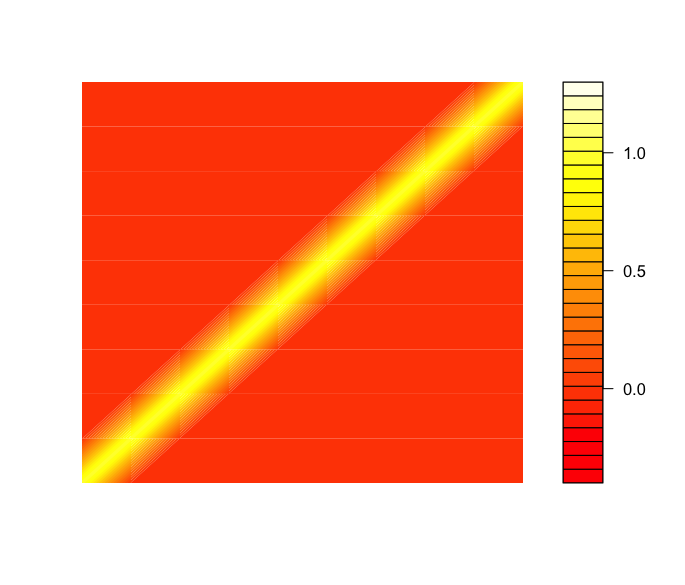
\includegraphics[width = .25\textwidth]{../img/chapter-4/true-covariance-1-heat-map}}%
%\subfigure{\label{fig:true-cov-2}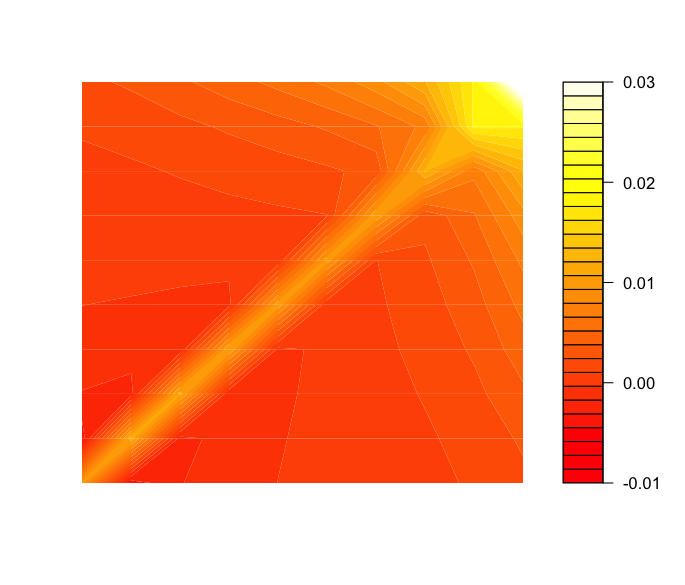
\includegraphics[width=0.25\textwidth]{../img/chapter-4/true-covariance-2-heat-map}}%
%\subfigure{\label{fig:true-cov-3}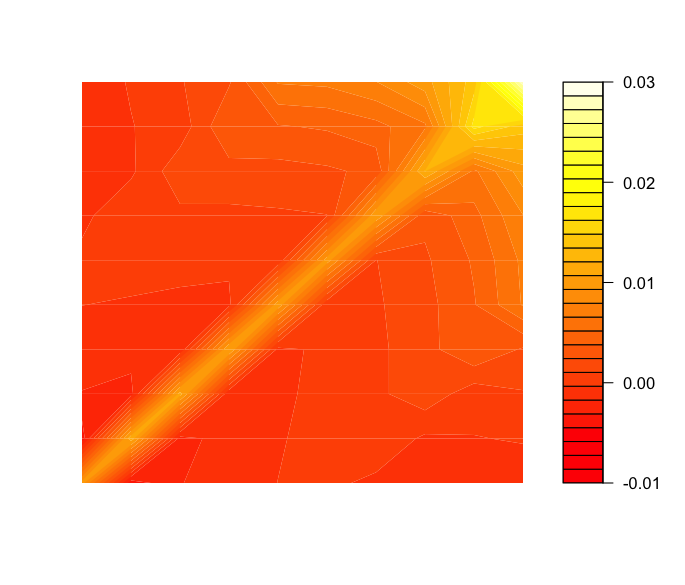
\includegraphics[width=0.25\textwidth]{../img/chapter-4/true-covariance-3-heat-map}}%
%\subfigure{\label{fig:true-cov-4}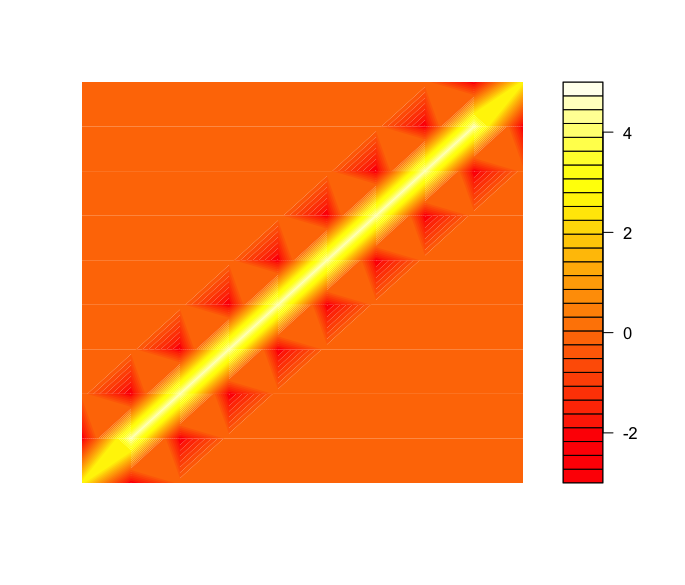
\includegraphics[width=0.25\textwidth]{../img/chapter-4/true-covariance-4-heat-map}}%
%\subfigure{\label{fig:true-cov-5}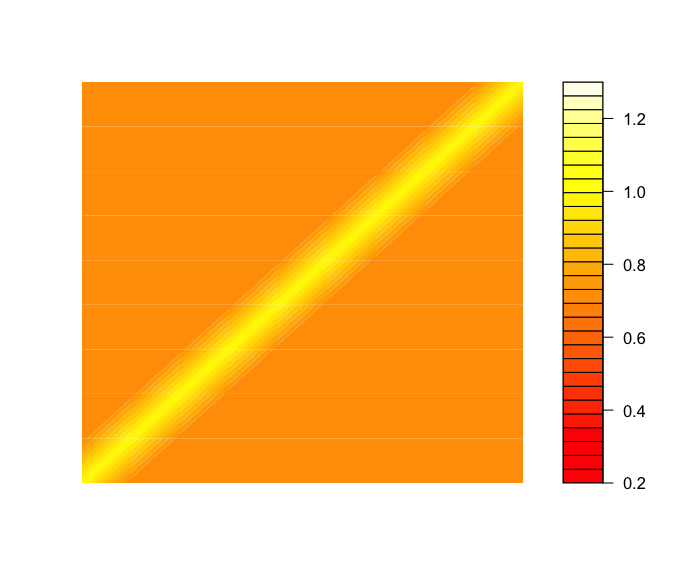
\includegraphics[width=0.25\textwidth]{../img/chapter-4/true-covariance-5-heat-map}} 
%}
%%\end{figure}
%%
%%\begin{figure}[H] \label{fig:oracle-surfaces-lattice}
%%\caption{Oracle estimates under models~\ref{item:cov-type-1} - \ref{item:cov-type-2}}
%\makebox[\linewidth][c]{%
%\centering
%\subfigure{\label{fig:oracle-cov-1}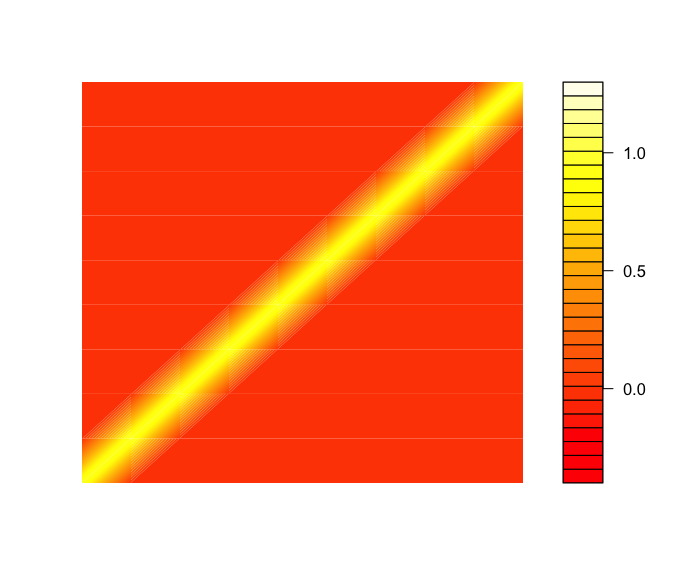
\includegraphics[width = .25\textwidth]{../img/chapter-4/oracle-covariance-1-heat-map}}
%\subfigure{\label{fig:oracle-cov-2}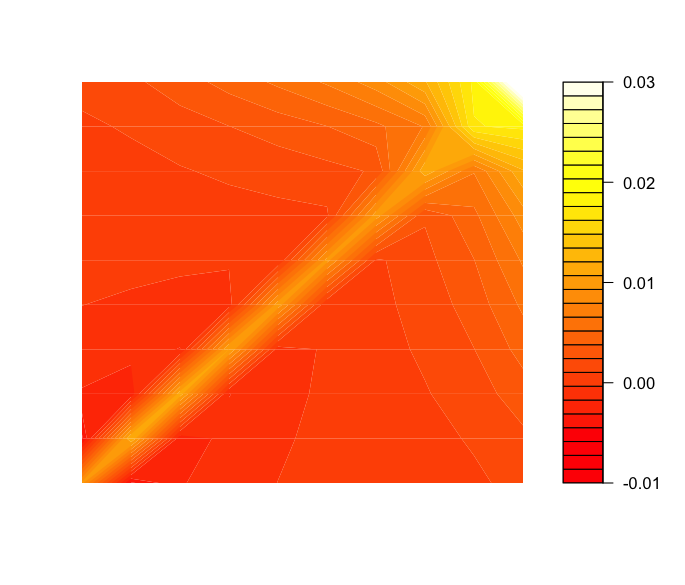
\includegraphics[width=0.25\textwidth]{../img/chapter-4/oracle-covariance-2-heat-map}}%
%\subfigure{\label{fig:oracle-cov-3}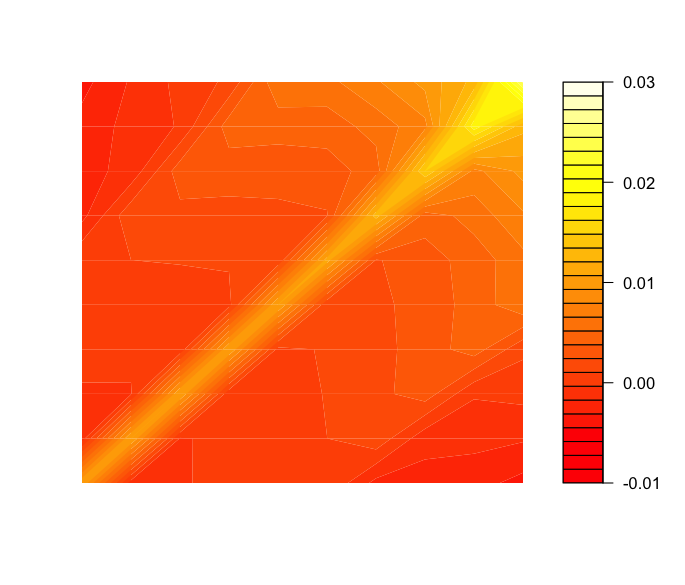
\includegraphics[width=0.25\textwidth]{../img/chapter-4/oracle-covariance-3-heat-map}}%
%\subfigure{\label{fig:oracle-cov-4}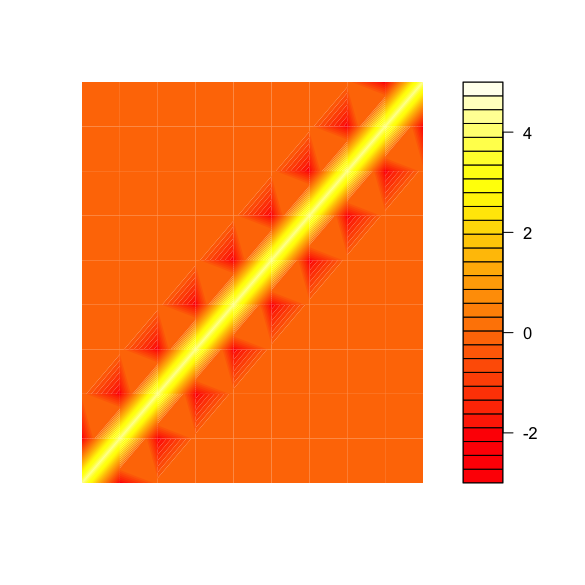
\includegraphics[width=0.25\textwidth]{../img/chapter-4/oracle-covariance-4-heat-map}}%
%\subfigure{\label{fig:oracle-cov-5}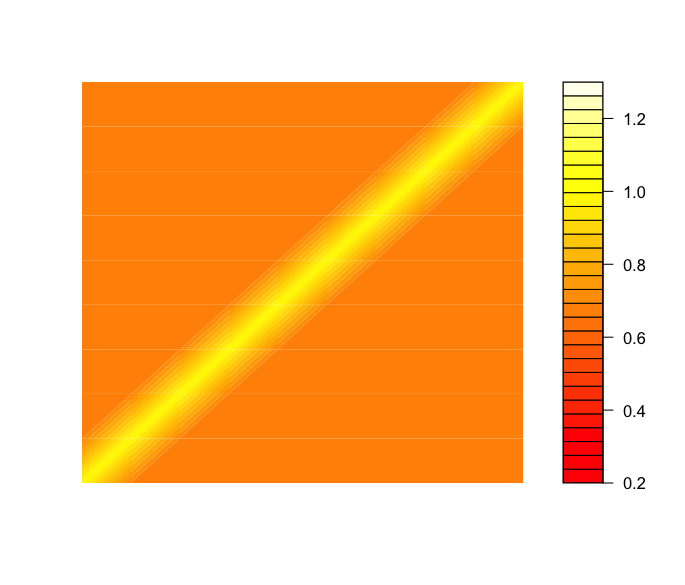
\includegraphics[width=0.25\textwidth]{../img/chapter-4/oracle-covariance-5-heat-map}}%
%}
%%\end{figure}
%%
%%\begin{figure}[H] \label{fig:true-cov-surfaces-lattice}
%%\caption{True covariance surfaces corresponding to Model~\ref{item:true-cov-1} - Model~\ref{item:true-cov-5}}
%\makebox[\linewidth][c]{%
%\centering
%\subfigure{\label{fig:ssanova-cov-1}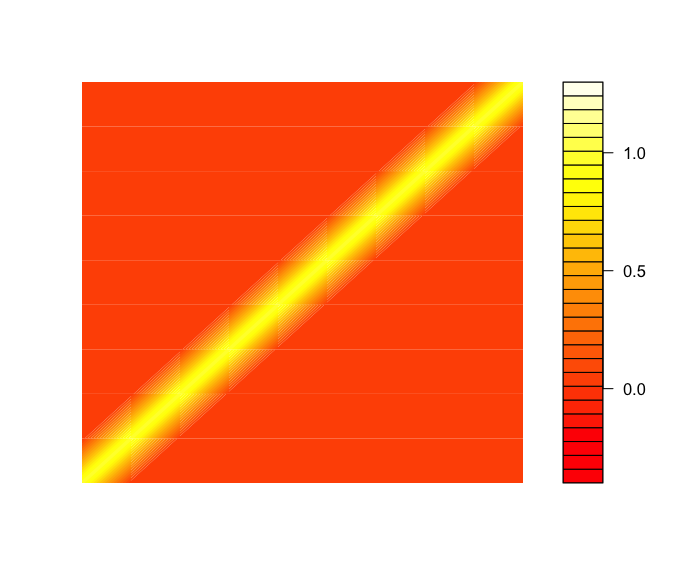
\includegraphics[width = .25\textwidth]{../img/chapter-4/ssanova-covariance-1-heat-map}}%
%\subfigure{\label{fig:ssanova-cov-2}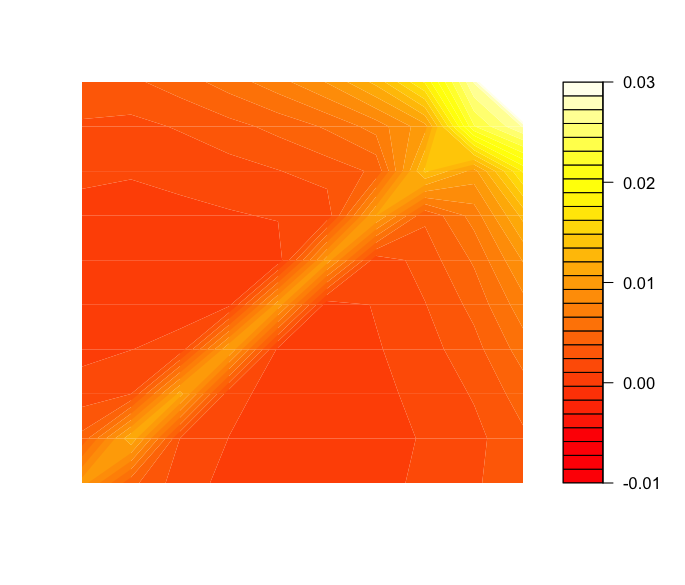
\includegraphics[width=0.25\textwidth]{../img/chapter-4/ssanova-covariance-2-heat-map}}%
%\subfigure{\label{fig:ssanova-cov-3}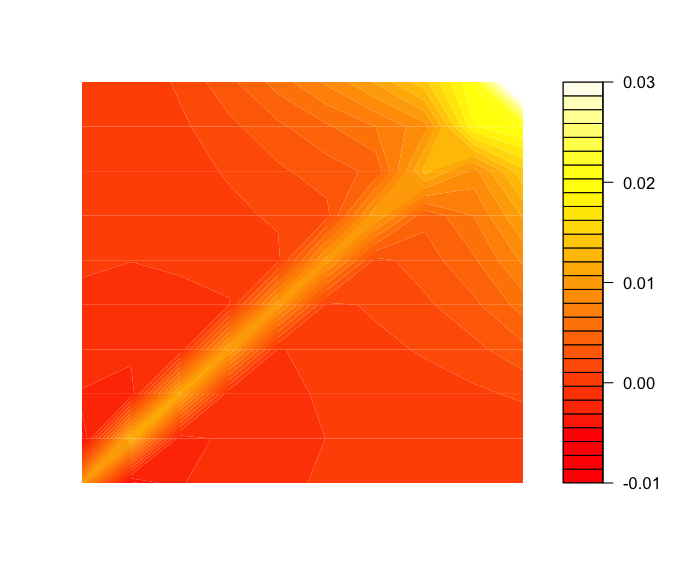
\includegraphics[width=0.25\textwidth]{../img/chapter-4/ssanova-covariance-3-heat-map}}%
%\subfigure{\label{fig:ssanova-cov-4}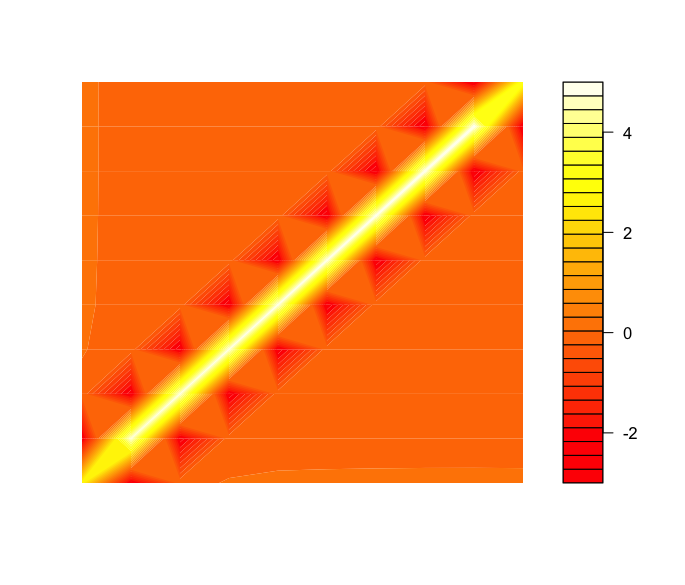
\includegraphics[width=0.25\textwidth]{../img/chapter-4/ssanova-covariance-4-heat-map}}%
%\subfigure{\label{fig:ssanova-cov-5}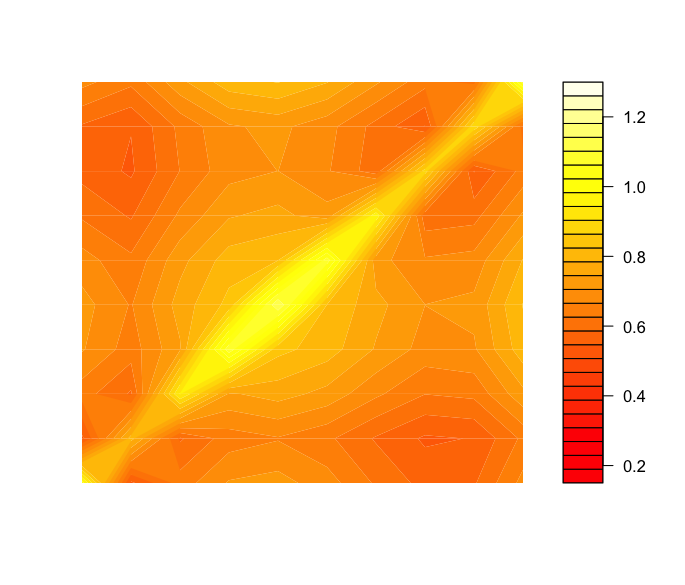
\includegraphics[width=0.25\textwidth]{../img/chapter-4/ssanova-covariance-5-heat-map}}%
%}
%\makebox[\linewidth][c]{%
%\centering
%\subfigure{\label{fig:polynomial-mcd-cov-1}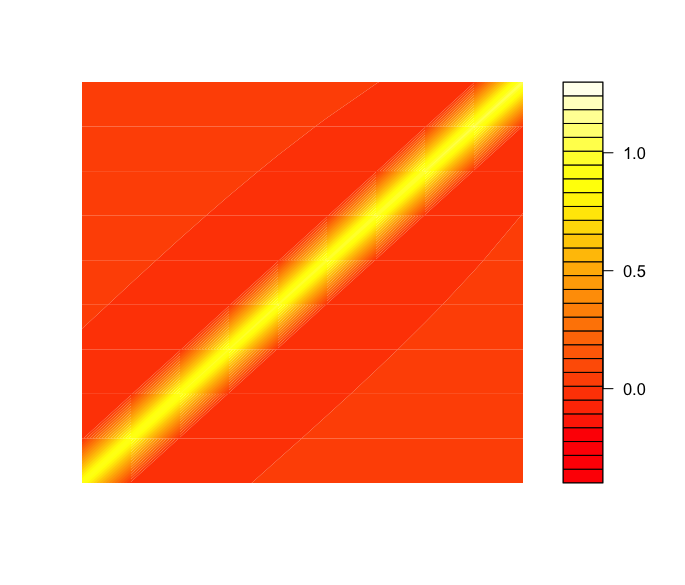
\includegraphics[width = .25\textwidth]{../img/chapter-4/polynomial-mcd-1-heat-map}}%
%\subfigure{\label{fig:polynomial-mcd-cov-2}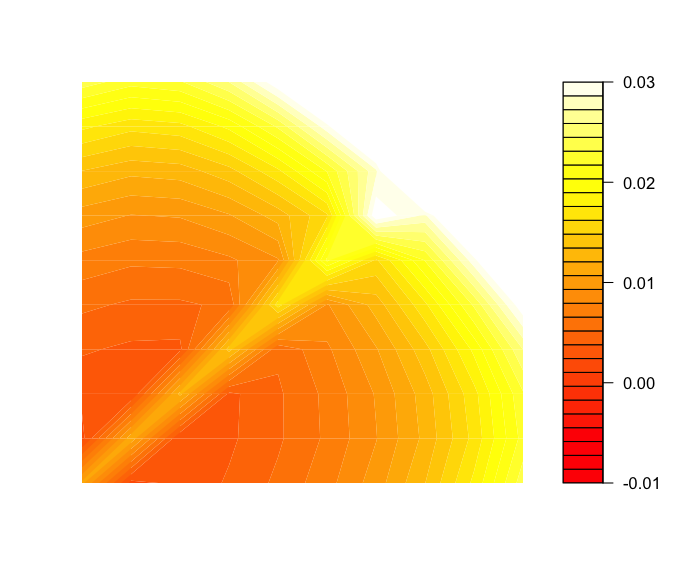
\includegraphics[width=0.25\textwidth]{../img/chapter-4/polynomial-mcd-2-heat-map}}%
%\subfigure{\label{fig:polynomial-mcd-cov-3}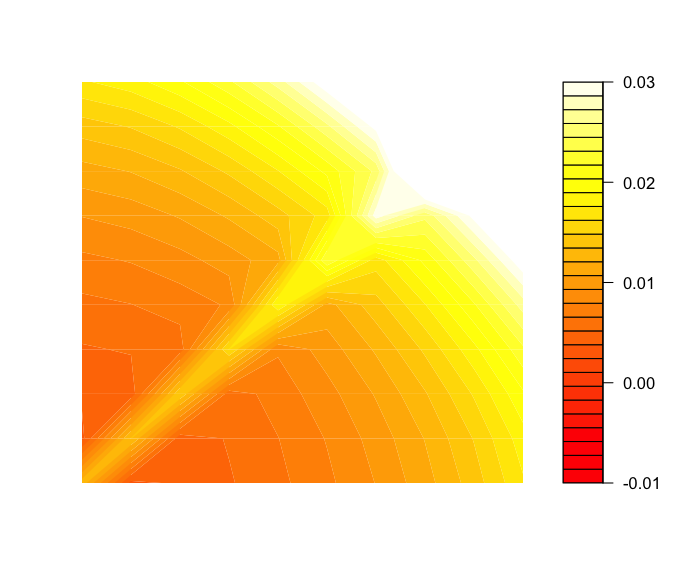
\includegraphics[width=0.25\textwidth]{../img/chapter-4/polynomial-mcd-3-heat-map}}%
%\subfigure{\label{fig:polynomial-mcd-cov-4}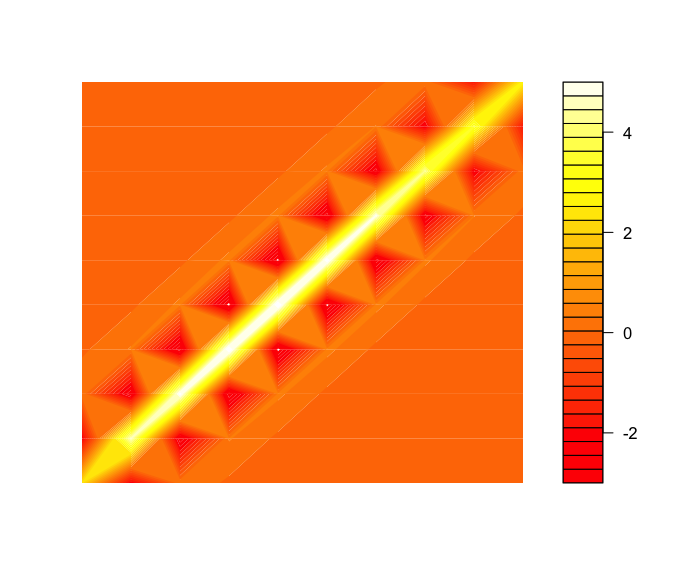
\includegraphics[width=0.25\textwidth]{../img/chapter-4/polynomial-mcd-4-heat-map}}%
%\subfigure{\label{fig:polynomial-mcd-cov-5}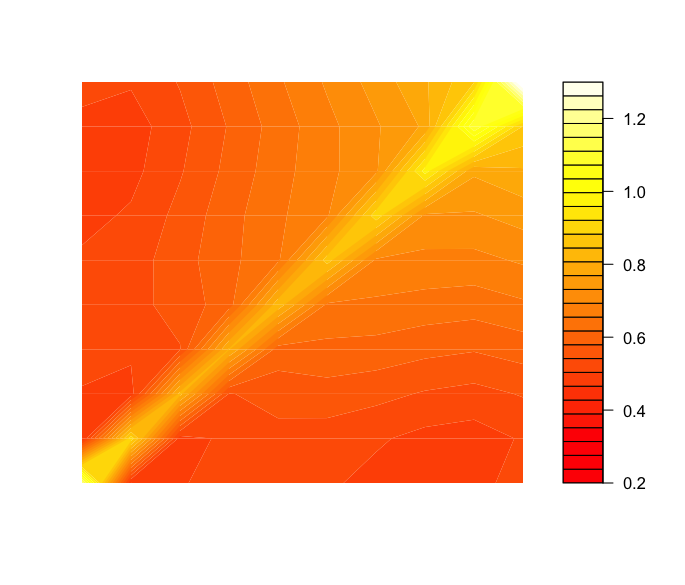
\includegraphics[width=0.25\textwidth]{../img/chapter-4/polynomial-mcd-5-heat-map}}%
%}
%%\makebox[\linewidth][c]{%
%%\centering
%%\subfigure{\label{fig:sample-cov-1}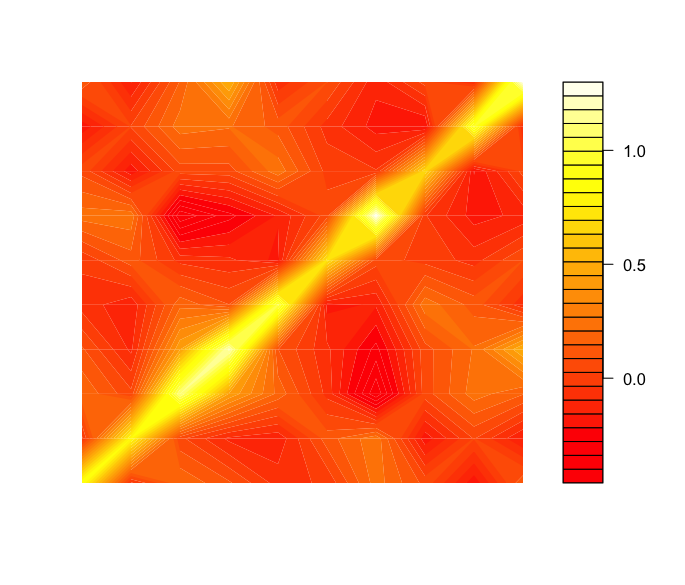
\includegraphics[width = .25\textwidth]{../img/chapter-4/sample-cov-1-heat-map}}%
%%\subfigure{\label{fig:sample-cov-2}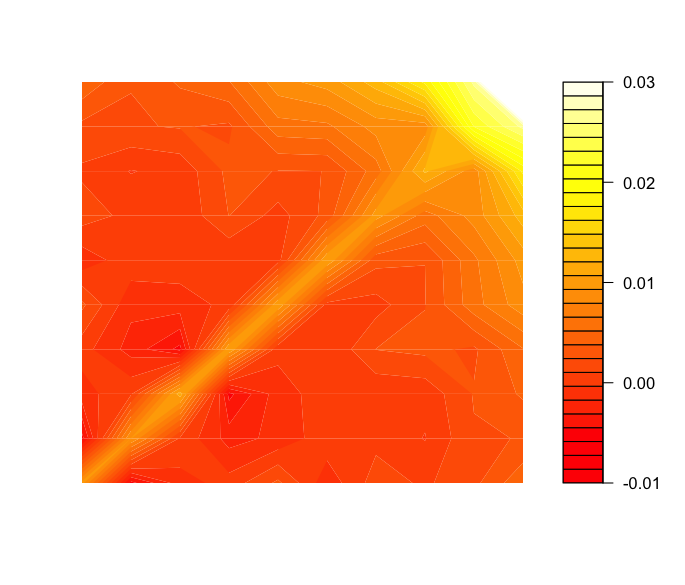
\includegraphics[width=0.25\textwidth]{../img/chapter-4/sample-cov-2-heat-map}}%
%%\subfigure{\label{fig:sample-cov-3}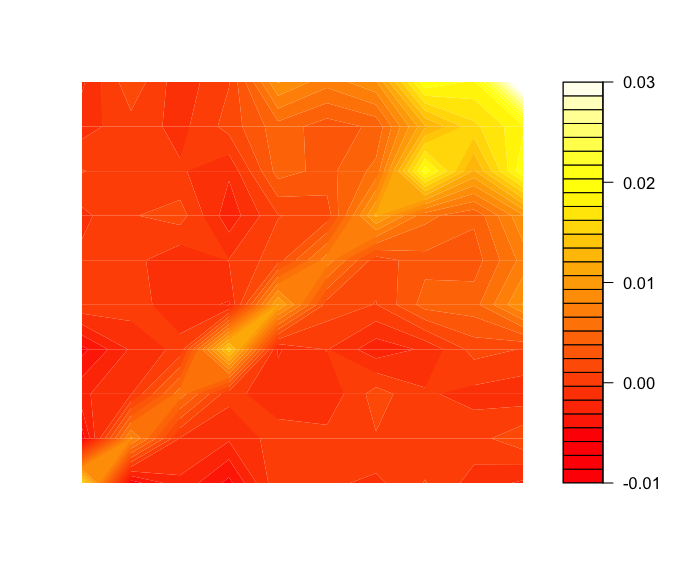
\includegraphics[width=0.25\textwidth]{../img/chapter-4/sample-cov-3-heat-map}}%
%%\subfigure{\label{fig:sample-cov-4}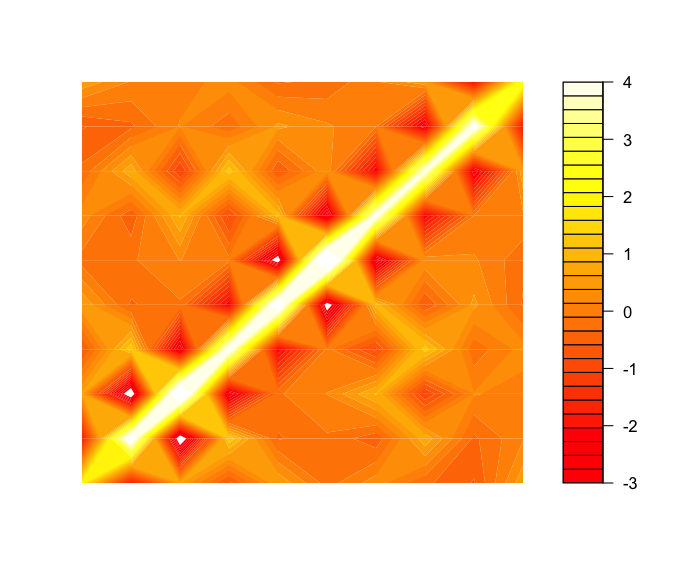
\includegraphics[width=0.25\textwidth]{../img/chapter-4/sample-cov-4-heat-map}}%
%%\subfigure{\label{fig:sample-cov-5}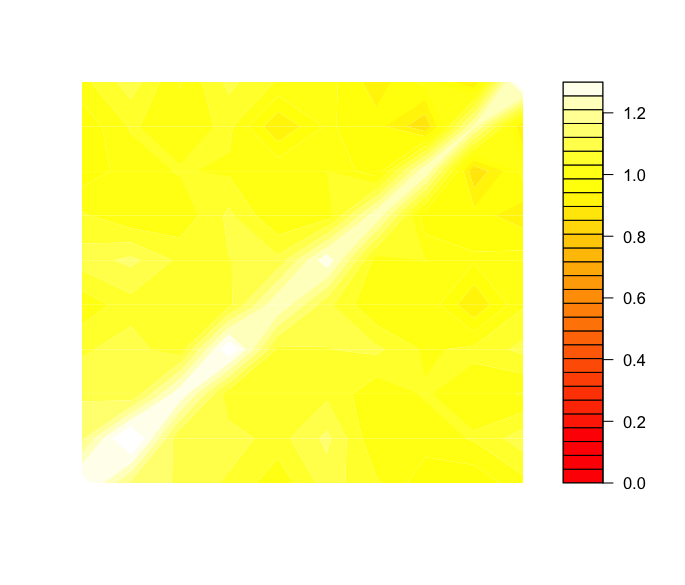
\includegraphics[width=0.25\textwidth]{../img/chapter-4/sample-cov-5-heat-map}}%
%%}
%%\makebox[\linewidth][c]{%
%%\centering
%%\subfigure{\label{fig:soft-thresholding-cov-1}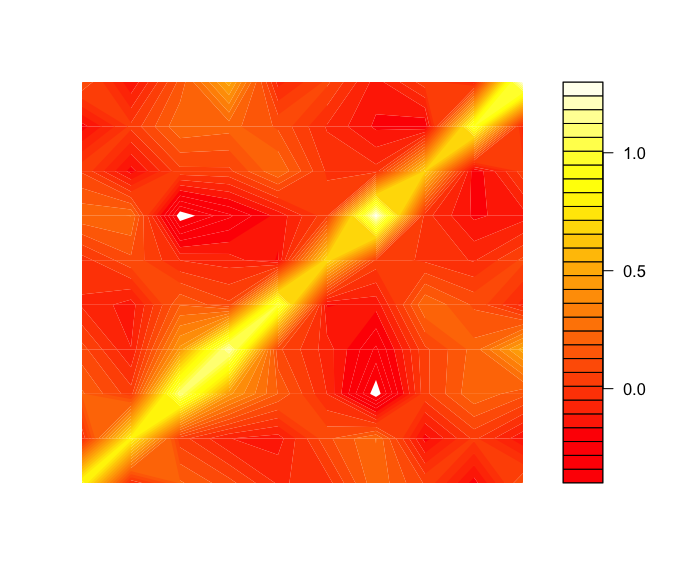
\includegraphics[width = .25\textwidth]{../img/chapter-4/soft-thresholding-1-heat-map}}%
%%\subfigure{\label{fig:soft-thresholding-cov-2}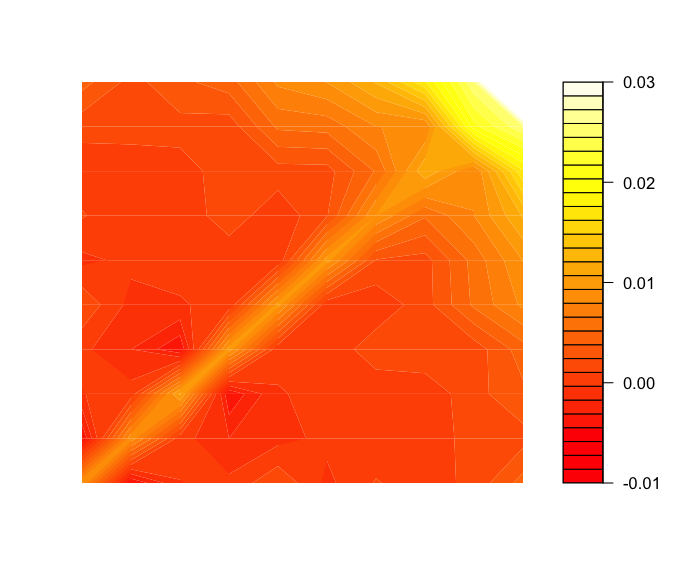
\includegraphics[width=0.25\textwidth]{../img/chapter-4/soft-thresholding-2-heat-map}}%
%%\subfigure{\label{fig:soft-thresholding-cov-3}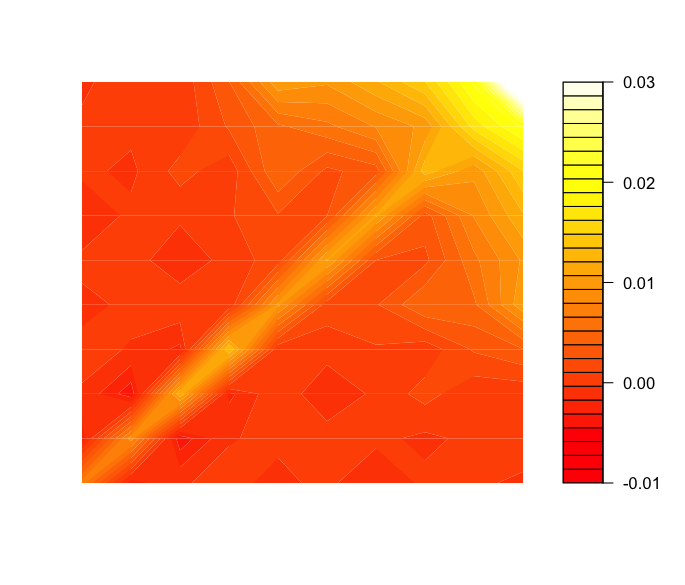
\includegraphics[width=0.25\textwidth]{../img/chapter-4/soft-thresholding-3-heat-map}}%
%%\subfigure{\label{fig:soft-thresholding-cov-4}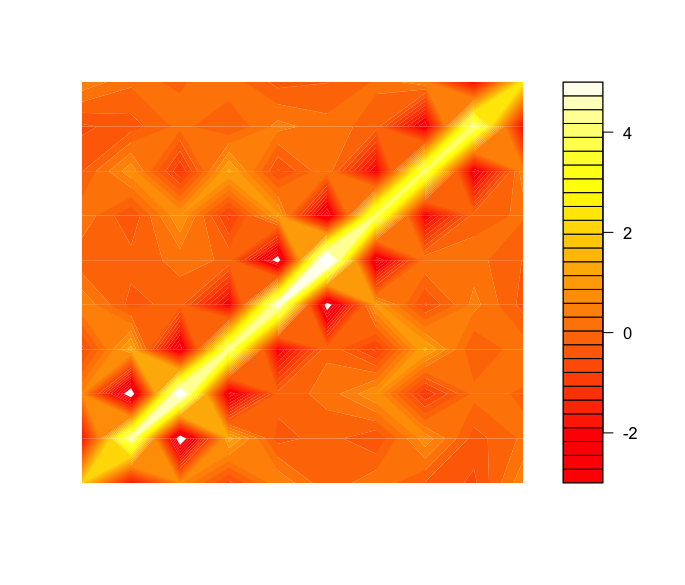
\includegraphics[width=0.25\textwidth]{../img/chapter-4/soft-thresholding-4-heat-map}}%
%%\subfigure{\label{fig:soft-thresholding-cov-5}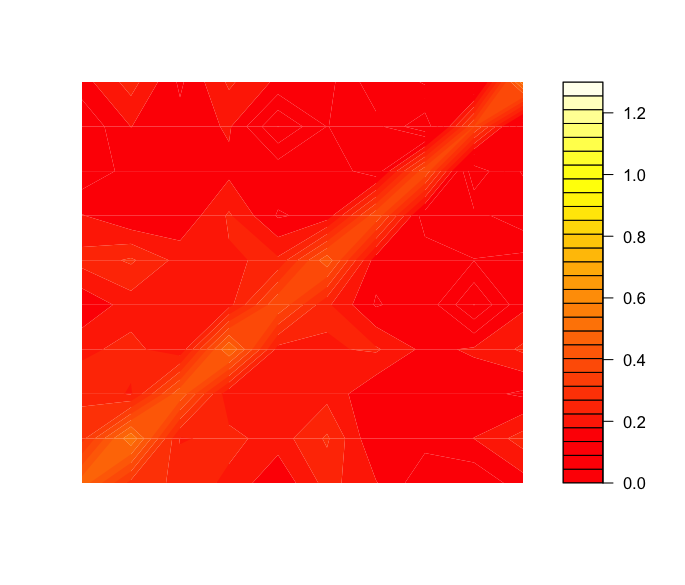
\includegraphics[width=0.25\textwidth]{../img/chapter-4/soft-thresholding-5-heat-map}}%
%%}
%%\makebox[\linewidth][c]{%
%%\centering
%%\subfigure{\label{fig:tapering-cov-1}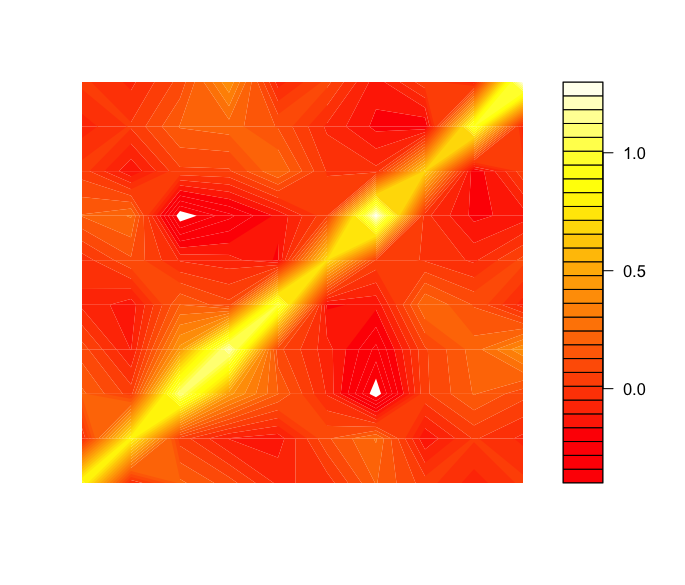
\includegraphics[width = .25\textwidth]{../img/chapter-4/tapering-estimator-1-heat-map}}%
%%\subfigure{\label{fig:tapering-cov-2}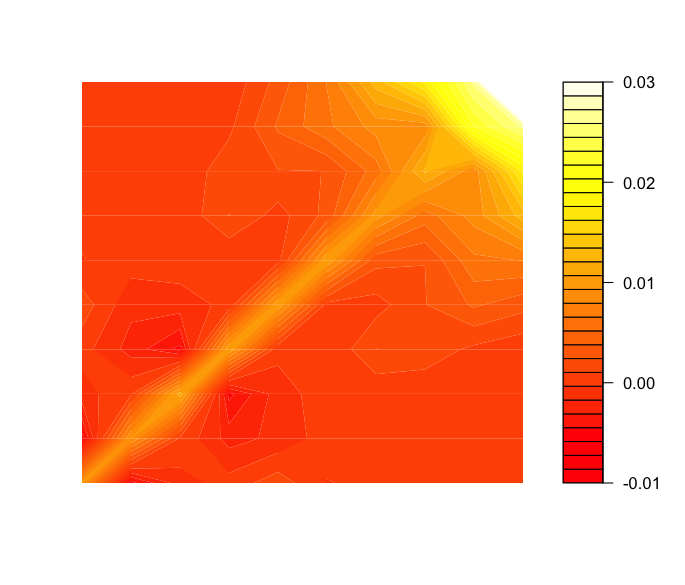
\includegraphics[width=0.25\textwidth]{../img/chapter-4/tapering-estimator-2-heat-map}}%
%%\subfigure{\label{fig:tapering-cov-3}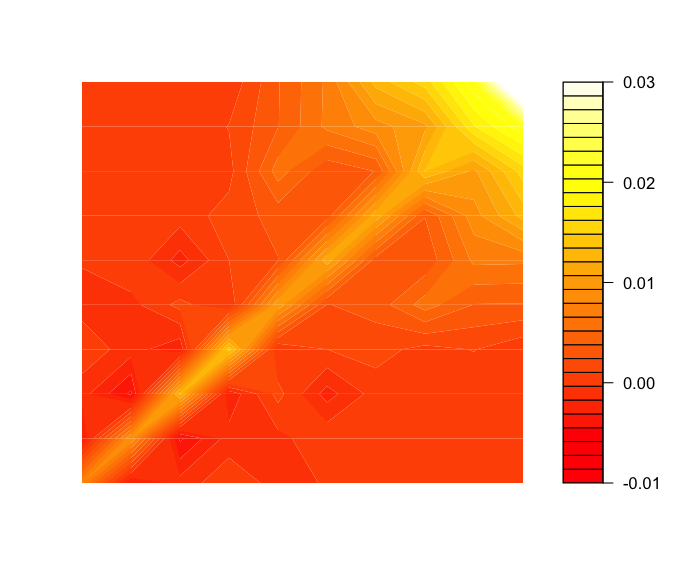
\includegraphics[width=0.25\textwidth]{../img/chapter-4/tapering-estimator-3-heat-map}}%
%%\subfigure{\label{fig:tapering-cov-4}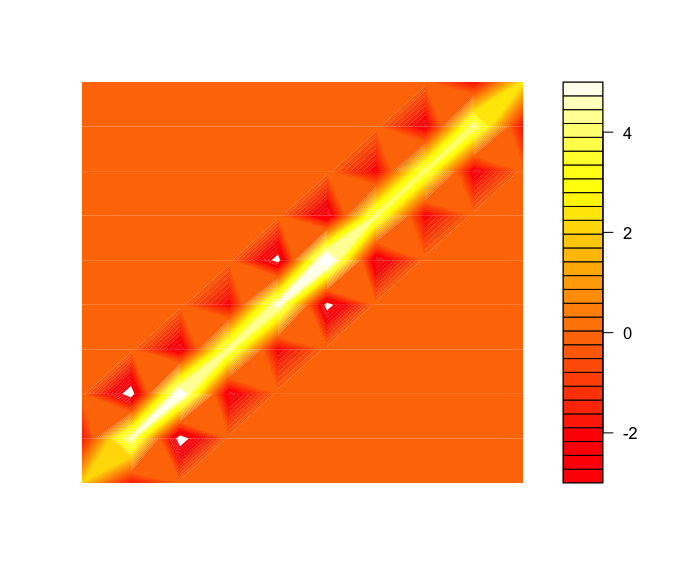
\includegraphics[width=0.25\textwidth]{../img/chapter-4/tapering-estimator-4-heat-map}}%
%%\subfigure{\label{fig:tapering-cov-5}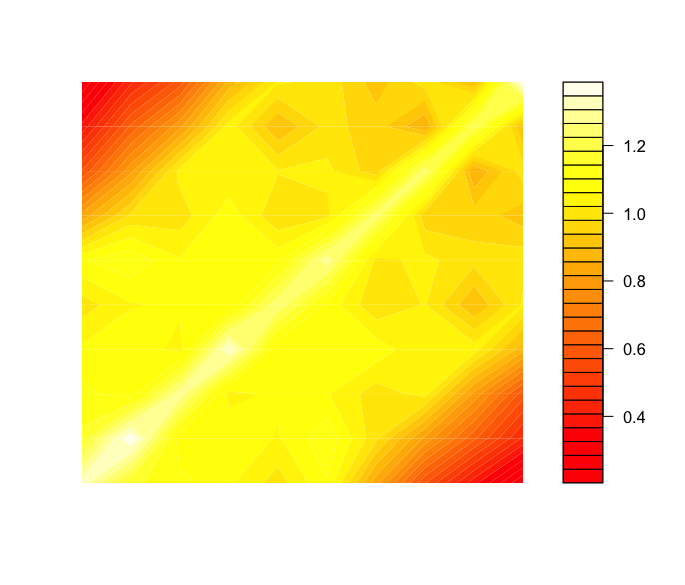
\includegraphics[width=0.25\textwidth]{../img/chapter-4/tapering-estimator-5-heat-map}}%
%%}
%\end{figure}
%



%
%\begin{figure}[H] \label{fig:true-cov-surfaces}
%\caption{True covariance surfaces corresponding to Model~\ref{item:true-cov-1} - Model~\ref{item:true-cov-5}}
%\makebox[\linewidth][c]{%
%\centering
%\subfigure{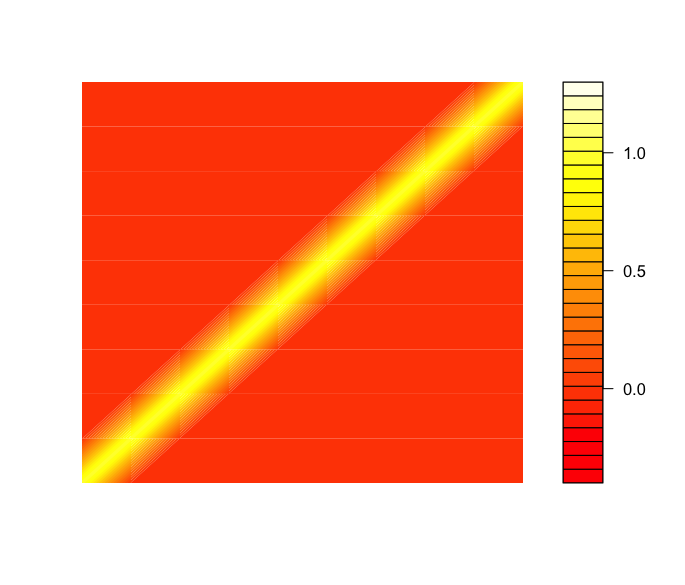
\includegraphics[width = .25\textwidth]{../img/chapter-4/true-covariance-1-heat-map}}%
%\subfigure{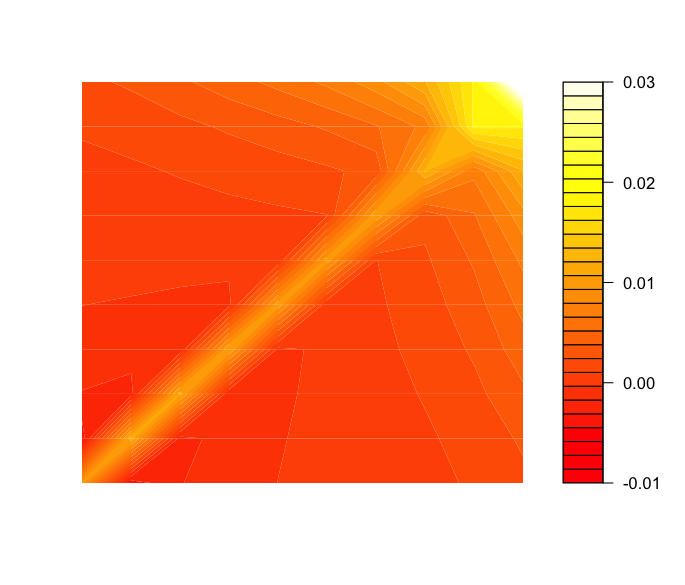
\includegraphics[width=0.25\textwidth]{../img/chapter-4/true-covariance-2-heat-map}}%
%\subfigure{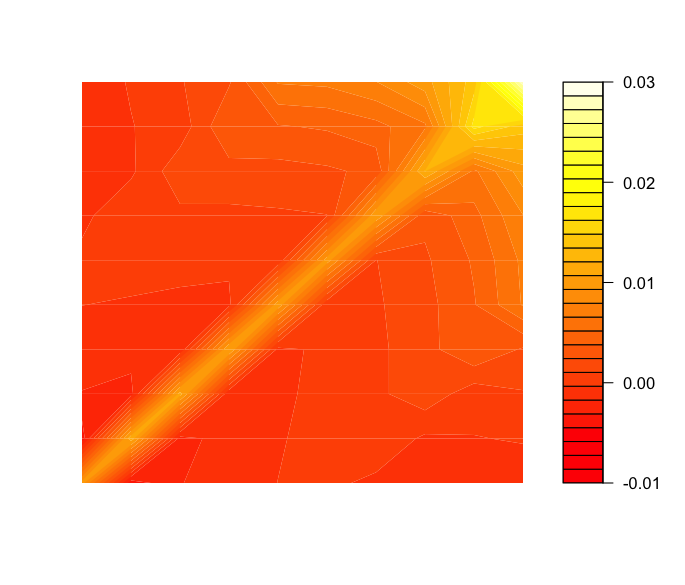
\includegraphics[width=0.25\textwidth]{../img/chapter-4/true-covariance-3-heat-map}}%
%\subfigure{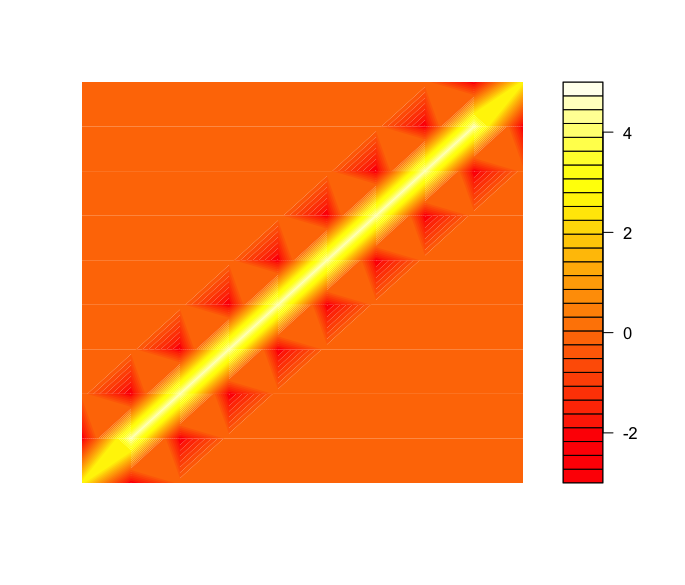
\includegraphics[width=0.25\textwidth]{../img/chapter-4/true-covariance-4-heat-map}}%
%\subfigure{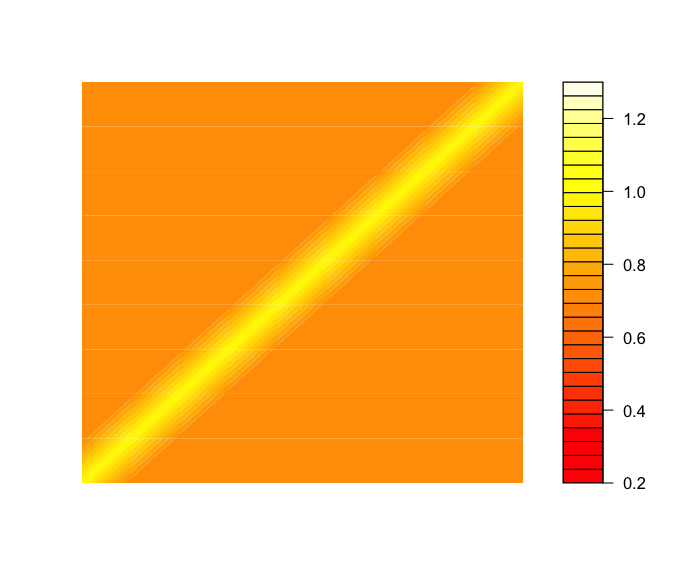
\includegraphics[width=0.25\textwidth]{../img/chapter-4/true-covariance-5-heat-map}}%
%}
%%\caption{Covariance structures used for data generation corresponding to models~\ref{item:cov-type-1} - \ref{item:cov-type-2}}
%%\makebox[\linewidth][c]{%
%%\centering
%%\subfigure[]{\label{fig:oracle-cov-1}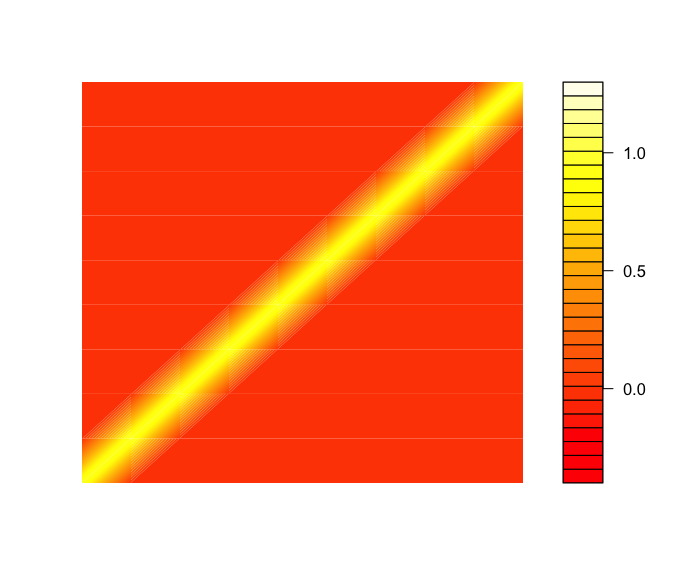
\includegraphics[width = .25\textwidth]{../img/chapter-4/oracle-covariance-1-heat-map}}%
%%\subfigure[]{\label{fig:oracle-cov-2}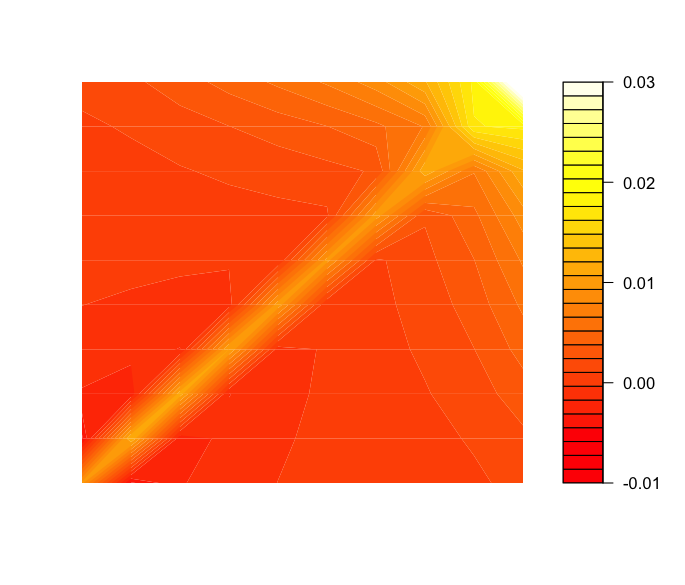
\includegraphics[width=0.25\textwidth]{../img/chapter-4/oracle-covariance-2-heat-map}}%
%%\subfigure[]{\label{fig:oracle-cov-3}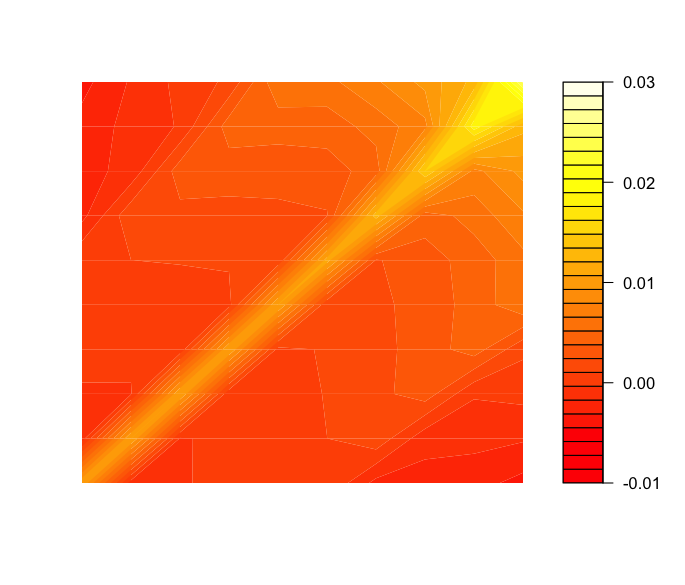
\includegraphics[width=0.25\textwidth]{../img/chapter-4/oracle-covariance-3-heat-map}}%
%%\subfigure[]{\label{fig:oracle-cov-4}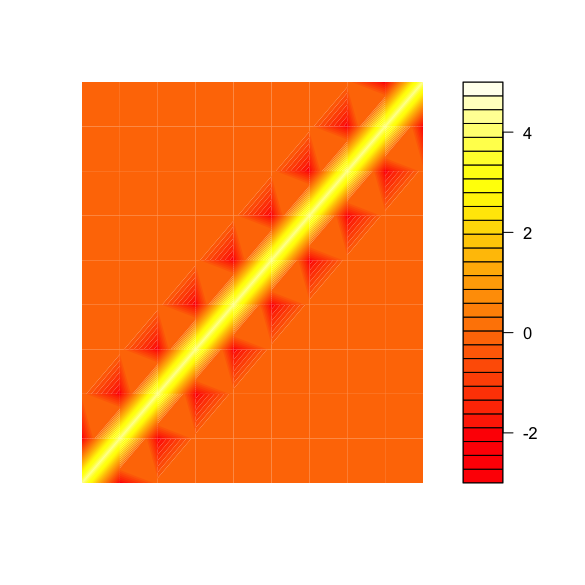
\includegraphics[width=0.25\textwidth]{../img/chapter-4/oracle-covariance-4-heat-map}}%
%%\subfigure[]{\label{fig:oracle-cov-5}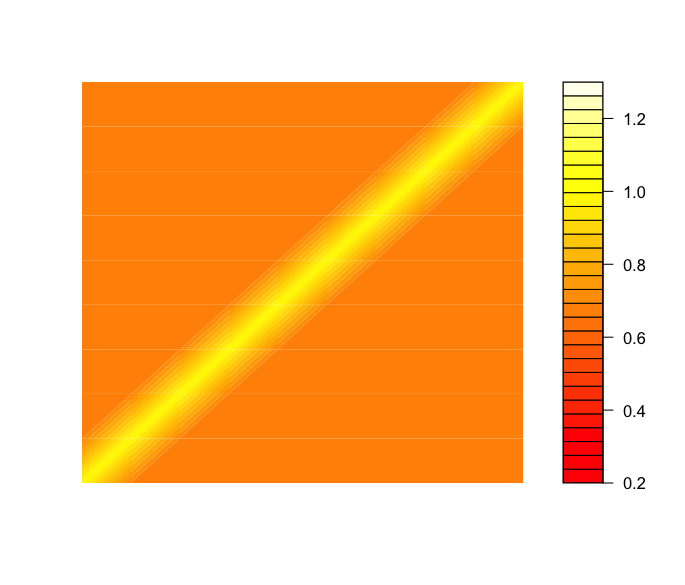
\includegraphics[width=0.25\textwidth]{../img/chapter-4/oracle-covariance-5-heat-map}}%
%%}
%%%\caption{Covariance structures used for data generation corresponding to models~\ref{item:cov-type-1} - \ref{item:cov-type-2}}
%%\makebox[\linewidth][c]{%
%%\centering
%%\subfigure{\label{fig:ssanova-cov-1}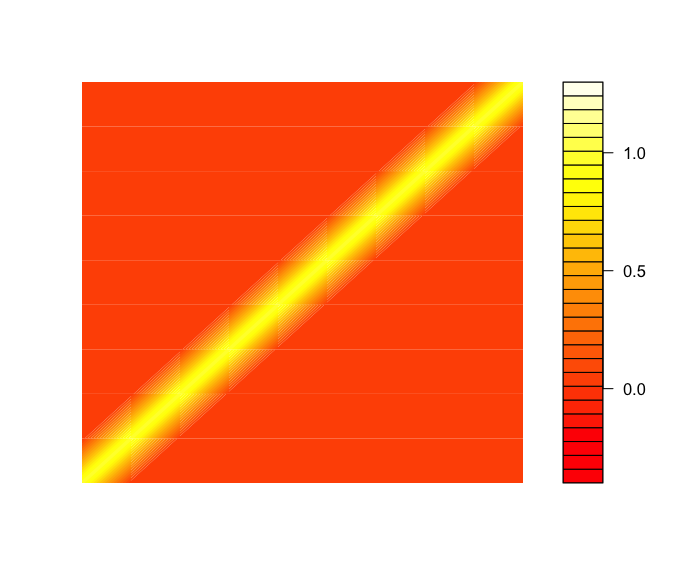
\includegraphics[width = .25\textwidth]{../img/chapter-4/ssanova-covariance-1-heat-map}}%
%%\subfigure{\label{fig:ssanova-cov-2}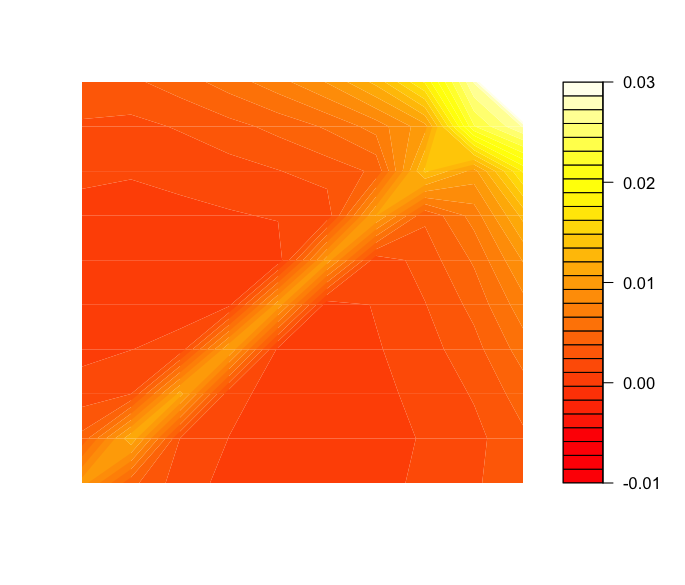
\includegraphics[width=0.25\textwidth]{../img/chapter-4/ssanova-covariance-2-heat-map}}%
%%\subfigure{\label{fig:ssanova-cov-3}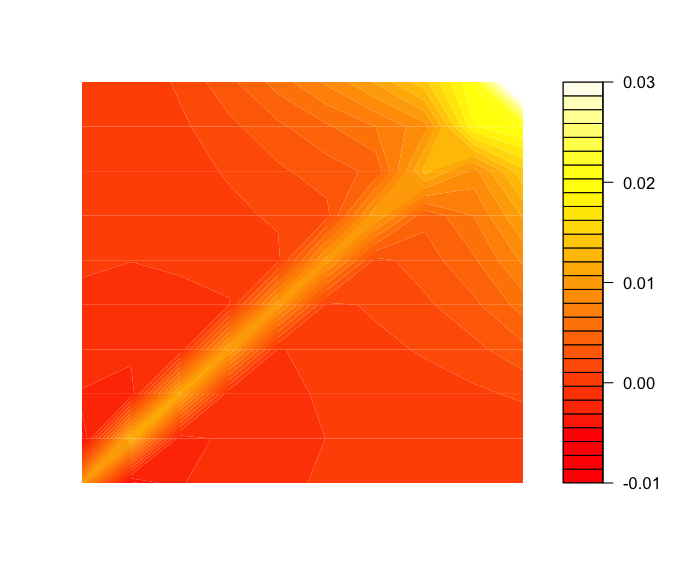
\includegraphics[width=0.25\textwidth]{../img/chapter-4/ssanova-covariance-3-heat-map}}%
%%\subfigure{\label{fig:ssanova-cov-4}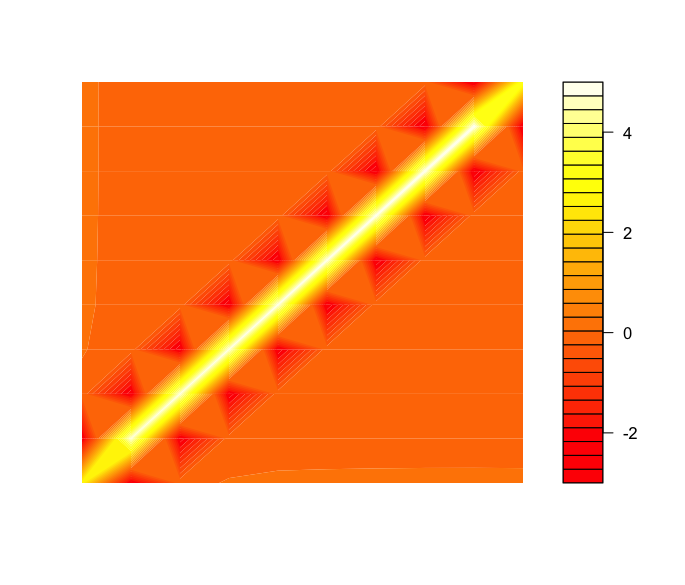
\includegraphics[width=0.25\textwidth]{../img/chapter-4/ssanova-covariance-4-heat-map}}%
%%\subfigure{\label{fig:ssanova-cov-5}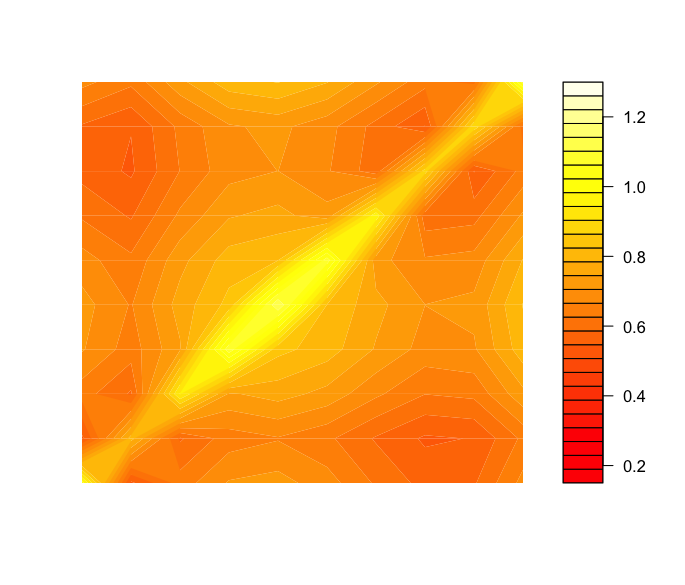
\includegraphics[width=0.25\textwidth]{../img/chapter-4/ssanova-covariance-5-heat-map}}%
%%}
%%\makebox[\linewidth][c]{%
%%\centering
%%\subfigure{\label{fig:polynomial-mcd-cov-1}\includegraphics[width = .25\textwidth]{../img/chapter-4/polynomial-mcd-1-heat-map}}%
%%\subfigure{\label{fig:polynomial-mcd-cov-2}\includegraphics[width=0.25\textwidth]{../img/chapter-4/polynomial-mcd-2-heat-map}}%
%%\subfigure{\label{fig:polynomial-mcd-cov-3}\includegraphics[width=0.25\textwidth]{../img/chapter-4/polynomial-mcd-3-heat-map}}%
%%\subfigure{\label{fig:polynomial-mcd-cov-4}\includegraphics[width=0.25\textwidth]{../img/chapter-4/polynomial-mcd-4-heat-map}}%
%%\subfigure{\label{fig:polynomial-mcd-cov-5}\includegraphics[width=0.25\textwidth]{../img/chapter-4/polynomial-mcd-5-heat-map}}%
%%}
%\makebox[\linewidth][c]{%
%\centering
%\subfigure{\label{fig:sample-cov-1}\includegraphics[width = .25\textwidth]{../img/chapter-4/sample-cov-1-heat-map}}%
%\subfigure{\label{fig:sample-cov-2}\includegraphics[width=0.25\textwidth]{../img/chapter-4/sample-cov-2-heat-map}}%
%\subfigure{\label{fig:sample-cov-3}\includegraphics[width=0.25\textwidth]{../img/chapter-4/sample-cov-3-heat-map}}%
%\subfigure{\label{fig:sample-cov-4}\includegraphics[width=0.25\textwidth]{../img/chapter-4/sample-cov-4-heat-map}}%
%\subfigure{\label{fig:sample-cov-5}\includegraphics[width=0.25\textwidth]{../img/chapter-4/sample-cov-5-heat-map}}%
%}
%\makebox[\linewidth][c]{%
%\centering
%\subfigure{\label{fig:soft-thresholding-cov-1}\includegraphics[width = .25\textwidth]{../img/chapter-4/soft-thresholding-1-heat-map}}%
%\subfigure{\label{fig:soft-thresholding-cov-2}\includegraphics[width=0.25\textwidth]{../img/chapter-4/soft-thresholding-2-heat-map}}%
%\subfigure{\label{fig:soft-thresholding-cov-3}\includegraphics[width=0.25\textwidth]{../img/chapter-4/soft-thresholding-3-heat-map}}%
%\subfigure{\label{fig:soft-thresholding-cov-4}\includegraphics[width=0.25\textwidth]{../img/chapter-4/soft-thresholding-4-heat-map}}%
%\subfigure{\label{fig:soft-thresholding-cov-5}\includegraphics[width=0.25\textwidth]{../img/chapter-4/soft-thresholding-5-heat-map}}%
%}
%\makebox[\linewidth][c]{%
%\centering
%\subfigure[Model I]{\label{fig:tapering-cov-1}\includegraphics[width = .25\textwidth]{../img/chapter-4/tapering-estimator-1-heat-map}}%
%\subfigure[Model II]{\label{fig:tapering-cov-2}\includegraphics[width=0.25\textwidth]{../img/chapter-4/tapering-estimator-2-heat-map}}%
%\subfigure[Model III]{\label{fig:tapering-cov-3}\includegraphics[width=0.25\textwidth]{../img/chapter-4/tapering-estimator-3-heat-map}}%
%\subfigure[Model IV]{\label{fig:tapering-cov-4}\includegraphics[width=0.25\textwidth]{../img/chapter-4/tapering-estimator-4-heat-map}}%
%\subfigure[Model V]{\label{fig:tapering-cov-5}\includegraphics[width=0.25\textwidth]{../img/chapter-4/tapering-estimator-5-heat-map}}%
%}
%\end{figure}


